\section{Results}

\subsection{Performance improved over time and did not differ between groups}

The average accuracy of BCI control increased from \metadataMeanAccuracyFirst~\% in the baseline session to \metadataMeanAccuracyLast~\% in the last session (Fig. \ref{fig:dataset_overview}A). Longitudinal changes were assessed with a linear mixed model, and the effect of session was statistically significant ($\beta = \metadataAccuracySessionBeta$, $t(\metadataAccuracySessionDf) = \metadataAccuracySessionTvalue, p \metadataAccuracySessionPvalue, 95\%~\text{CI:}~ [\metadataAccuracySessionBetaCIMin,$ $\metadataAccuracySessionBetaCIMax]$). As shown in the previous analyses of the same dataset \citep{Stieger2020_analysis}, there were no significant differences in the mean accuracy between MBSR (\metadataMeanAccuracyMBSR~\%) and control (\metadataMeanAccuracyControl~\%) groups: $t(\metadataGroupDiffDf) = \metadataGroupDiffTvalue, p \metadataGroupDiffPvalue, \text{Cohen's}~d = \metadataGroupDiffCohensD, 95\% ~\text{CI of the difference}~\allowbreak[\metadataGroupDiffCIMin,  \metadataGroupDiffCIMax]$ (Fig. \ref{fig:dataset_overview}B). The mean accuracy of all participants was \metadataMeanAccuracy\%. At the same time, the intra-individual variability of performance was quite considerable (Fig. \ref{fig:dataset_overview}C). We used linear mixed models to account for this variability in the current analysis.

\begin{figure}[htbp]
    \centering
    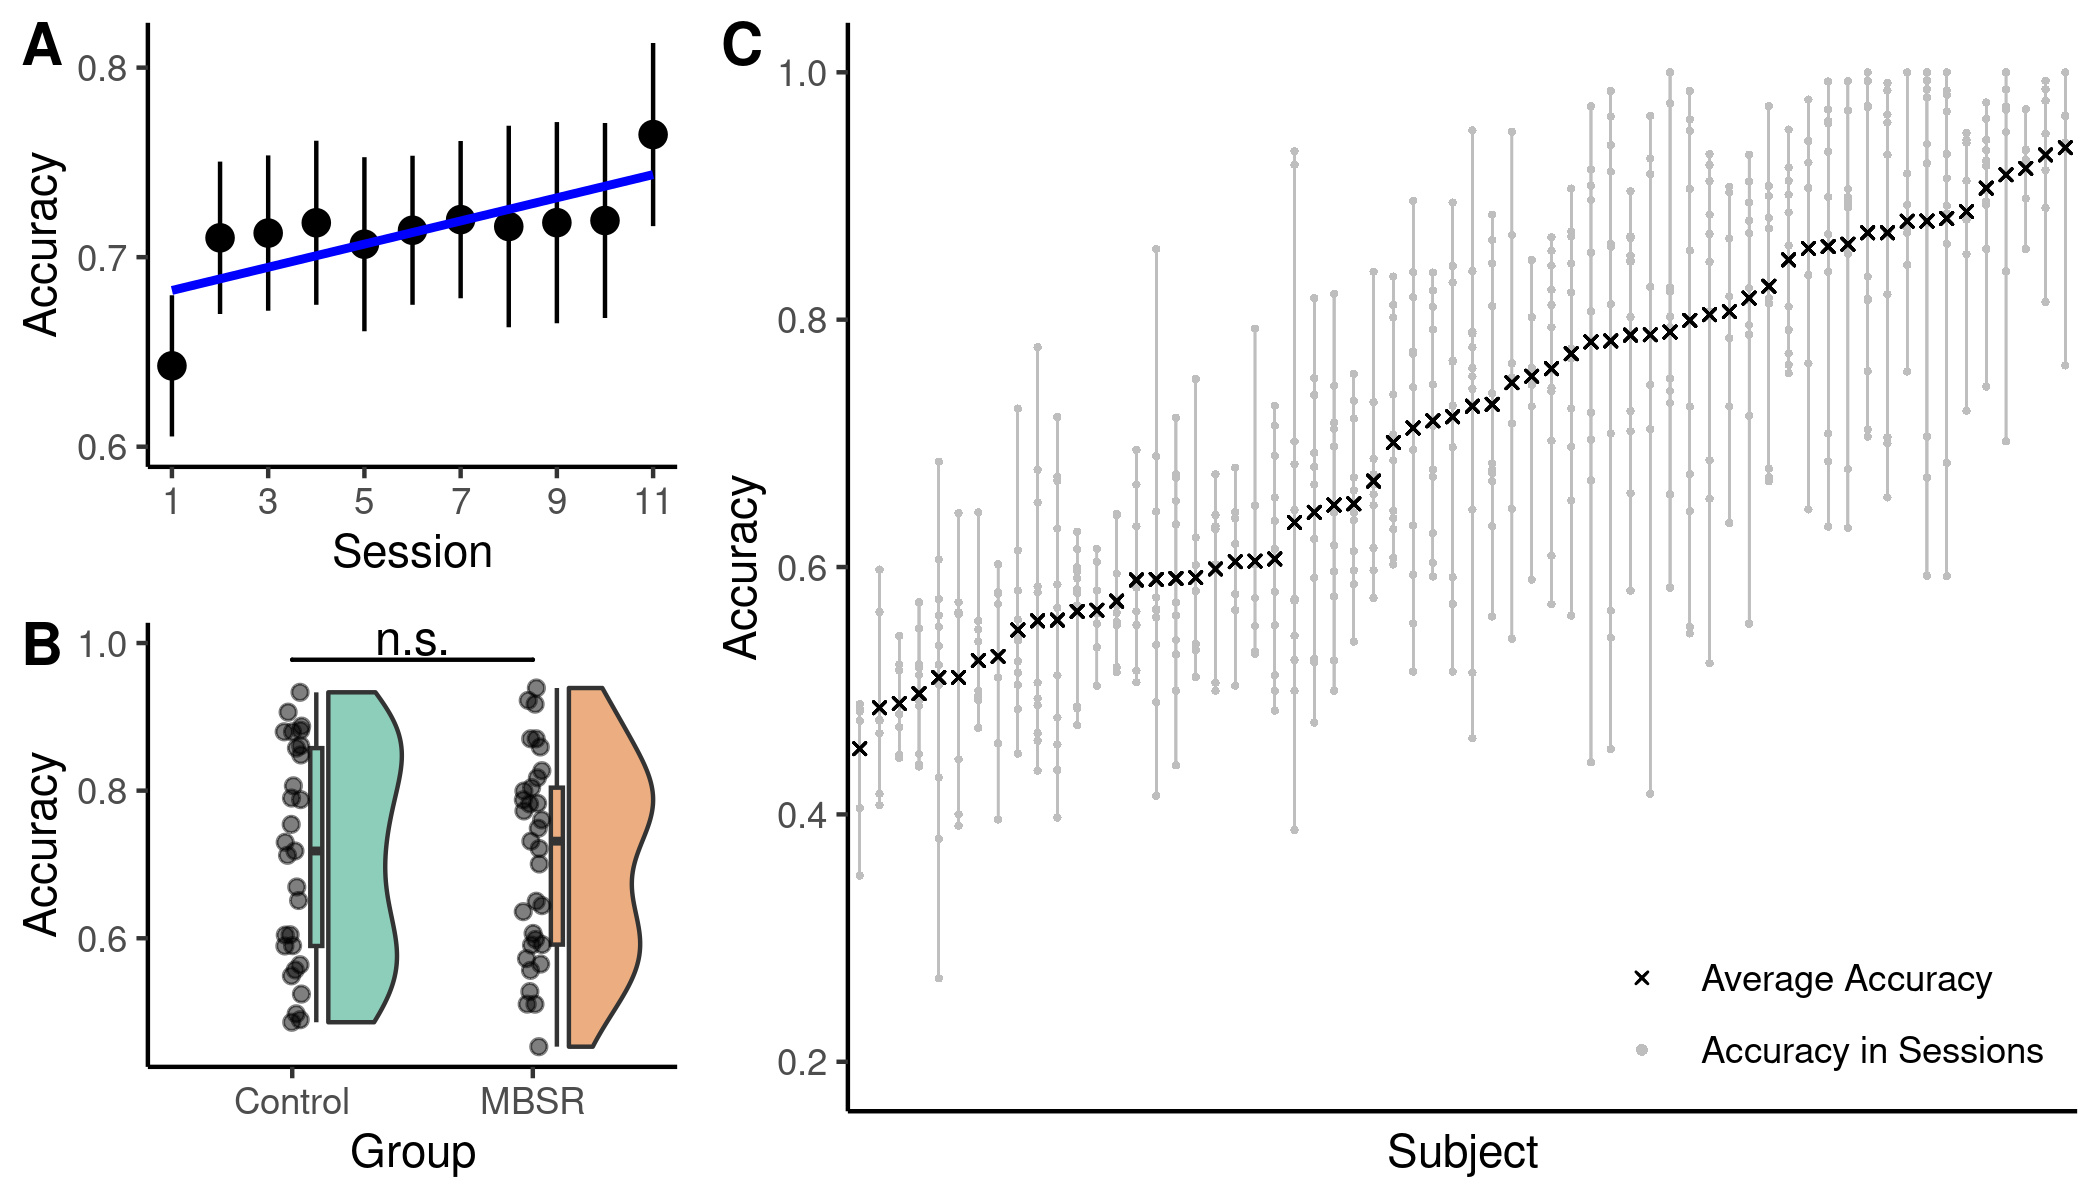
\includegraphics[width=\textwidth]{fig3-accuracy.png}
    \caption{Performance of the participants improved throughout the BCI training and showed high between- and within-subject variability. (A) Dynamics of group-average performance reflect improvement over the course of the training. Error bars reflect the standard error of the mean. (B) No difference in average performance in the horizontal cursor control task was observed between the MBSR (mindfulness-based stress reduction) and control groups. (C) High variability of performance in the individual sessions was observed and accounted for in the analyses. Subjects are ordered according to their average accuracy. Vertical bars depict subject-specific ranges of accuracy.}
    \label{fig:dataset_overview}
\end{figure}

\subsection{Sensorimotor ROIs contained the majority of task-relevant sources}

For some of the source space analysis pipelines, we identified the task-relevant sources by fitting CSP to distinguish between imaginary movements of two hands. For this purpose, we used EEG during the target presentation interval as it showed a difference in mu power between the imaginary movements primarily over the sensorimotor areas (Fig. \ref{fig:study_overview}C). The resulting CSP patterns and the corresponding power spectra for left- and right-hand movements are shown in Fig. \ref{fig:group_csp_source_space_mask}A and Fig. \ref{fig:group_csp_source_space_mask}B, respectively. These patterns were source reconstructed with eLORETA to assess the contribution of individual sources to CSP components (Fig. \ref{fig:group_csp_source_space_mask}C). Sources that exceeded the \cspSourceThreshold th percentile of activity strength were considered task-relevant, and Tab. \ref{supp-tab:csp_sources_per_roi} shows that the sensorimotor ROIs contained the highest number of selected sources. Task-relevant sources formed the resulting source mask (Fig. \ref{fig:group_csp_source_space_mask}D), which was applied to the anatomical definitions of sensorimotor ROIs to obtain a task-based reduced representation (Fig. \ref{fig:pipeline_overview}B).

\begin{figure}[htbp]
    \centering
    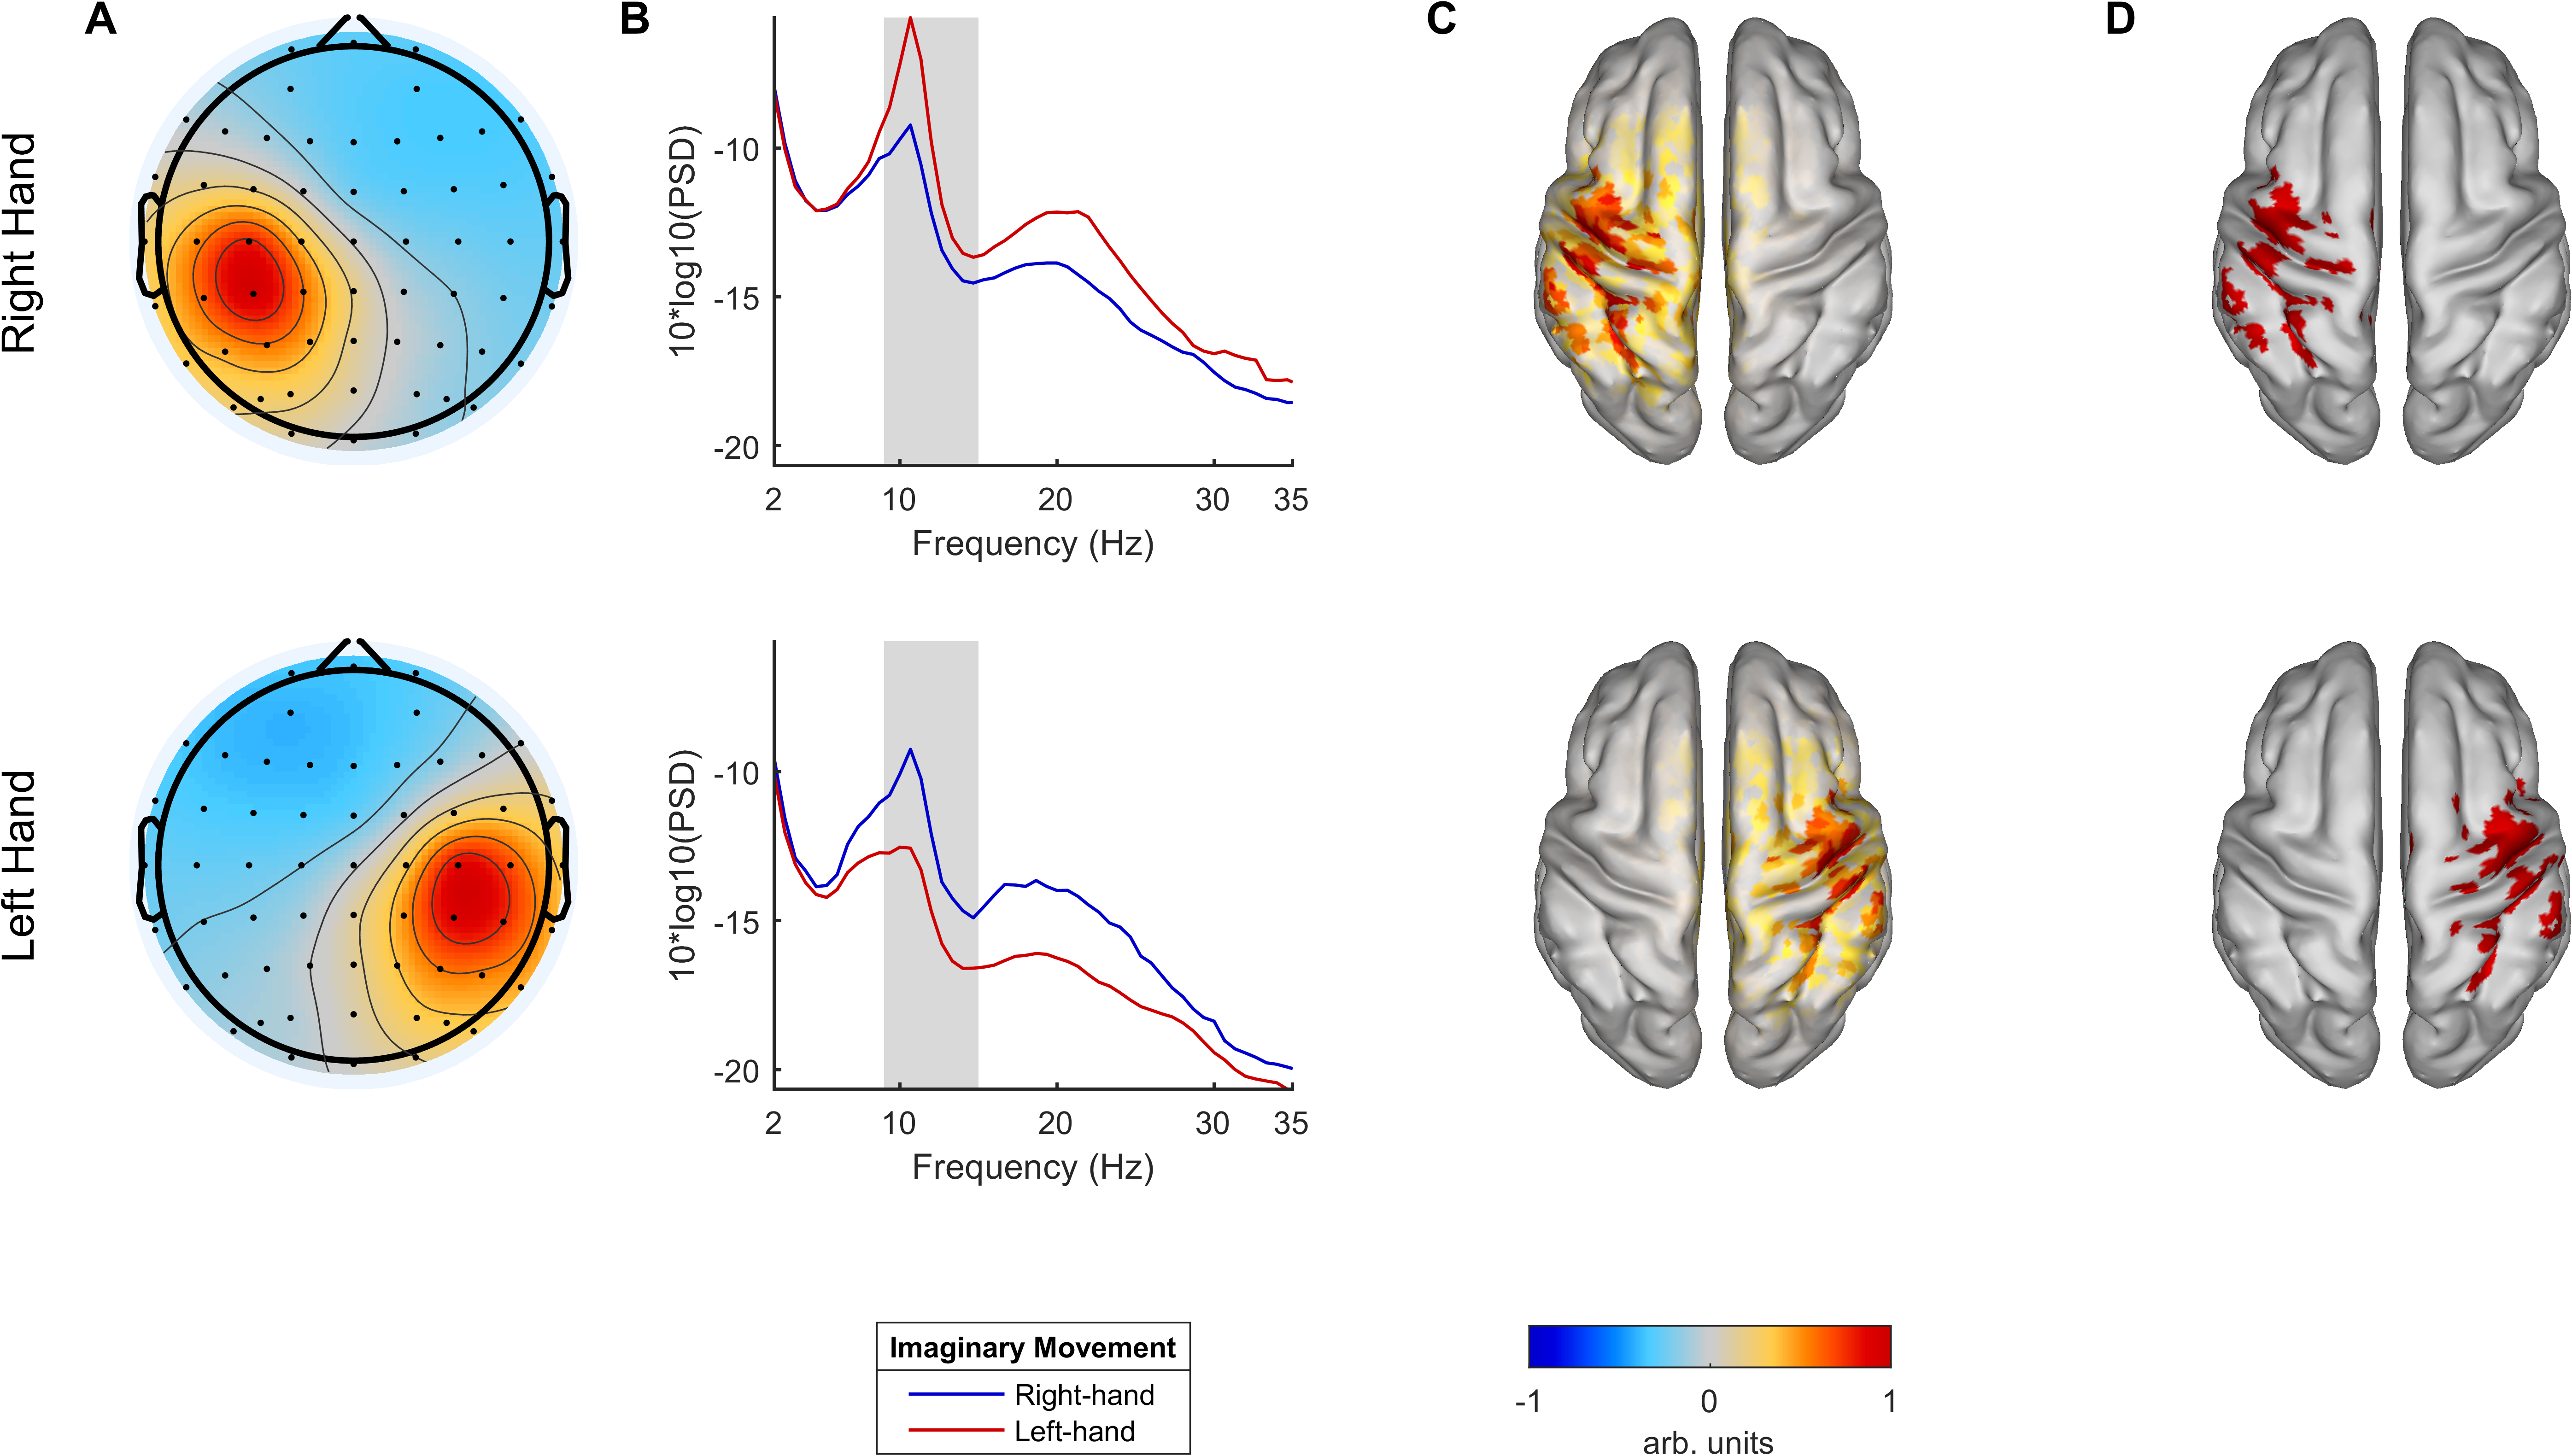
\includegraphics[width=\textwidth]{fig4-group-csp-source-space-mask.png}
    \caption{The task-relevant sources were identified through applying CSP to the EEG data during the target presentation interval after filtering in the \muLow-\muHigh~Hz frequency band. (A) Spatial patterns corresponding to the CSP filters that best discriminate imaginary movements of the right (upper row) and left (lower row) hands. Values were scaled to the [-1, 1] range. (B) Grand average power spectra of the CSP components corresponding to the spatial patterns from (A). The shaded area depicts the \muLow-\muHigh~Hz frequency band that was used to fit CSP. (C) Source reconstruction (absolute values, scaled to [-1, 1] range) of the spatial patterns from (A) with eLORETA. (D) Sources that exceeded the \cspSourceThreshold th percentile of activity strength were considered the most relevant for the execution of the motor imagery task.}
    \label{fig:group_csp_source_space_mask}
\end{figure}

\subsection{Laplace SNR was correlated with BCI performance but did not change across experimental sessions}

In the Laplacian-based analysis, we estimated the effects of SNR and phase synchronization (PS; see Supplementary Material, Section \ref{supp-sec:laplace_connectivity}) on BCI performance and their longitudinal changes. We used FOOOF to estimate average values of SNR at the Laplace-filtered channels C3 and C4. Examples of average power spectra for three representative subjects with different levels of Laplace SNR are shown in Fig. \ref{fig:snr_vs_accuracy_session_combined}A. Similar to performance, Laplace SNR did not differ significantly between the participant groups as shown in Fig. \ref{fig:snr_vs_accuracy_session_combined}B ($t(\laplaceGroupDiffSNRDf) = \laplaceGroupDiffSNRTvalue, p \laplaceGroupDiffSNRPvalue, \text{Cohen's}~d = \laplaceGroupDiffSNRCohensD, 95\%~\text{CI of the difference:}~ [\laplaceGroupDiffSNRCIMin, \laplaceGroupDiffSNRCIMax]$). Dynamics of the group-average Laplace SNR across experimental sessions are shown in Fig. \ref{fig:snr_vs_accuracy_session_combined}C.

\medskip

Similar to \citep{Blankertz2010}, we checked whether Laplace SNR was related to successful performance in the BCI training. Subject-average values of Laplace SNR were positively correlated with accuracy ($r=\laplaceSubjectAverageSNRrestAccuracyCor, t(\laplaceSubjectAverageSNRrestAccuracyDf) = \laplaceSubjectAverageSNRrestAccuracyTvalue, p \laplaceSubjectAverageSNRrestAccuracyPvalue, 95\%~\text{CI:}~ [\laplaceSubjectAverageSNRrestAccuracyCIMin, \laplaceSubjectAverageSNRrestAccuracyCIMax]$), showing a between-subject effect of Laplace SNR on performance (Fig. \ref{fig:snr_vs_accuracy_session_combined}D). Additionally, the within-subject effect of Laplace SNR on accuracy was significant, as assessed with a linear mixed model ($\beta = \laplaceWithinSubjectSNRrestAccuracyBeta, t(\laplaceWithinSubjectSNRrestAccuracyDf) = \laplaceWithinSubjectSNRrestAccuracyTvalue, p \laplaceWithinSubjectSNRrestAccuracyPvalue, 95\%~\text{CI:}~ [\laplaceWithinSubjectSNRrestAccuracyBetaCIMin, \laplaceWithinSubjectSNRrestAccuracyBetaCIMax]$). Figure \ref{fig:snr_vs_accuracy_session_combined}E illustrates the observed within-subject effect.

\medskip

Then, we investigated whether Laplace SNR changed over time due to the training, but longitudinal changes were not significant ($\beta = \laplaceWithinSubjectSNRrestSessionBeta, t(\laplaceWithinSubjectSNRrestSessionDf) = \laplaceWithinSubjectSNRrestSessionTvalue, p \laplaceWithinSubjectSNRrestSessionPvalue, 95\%~\text{CI:}\allowbreak[\laplaceWithinSubjectSNRrestSessionBetaCIMin, \laplaceWithinSubjectSNRrestSessionBetaCIMax]$). Individual and group-level trends are shown in Fig. \ref{fig:snr_vs_accuracy_session_combined}F.

\begin{figure}[htbp]
    \centering
    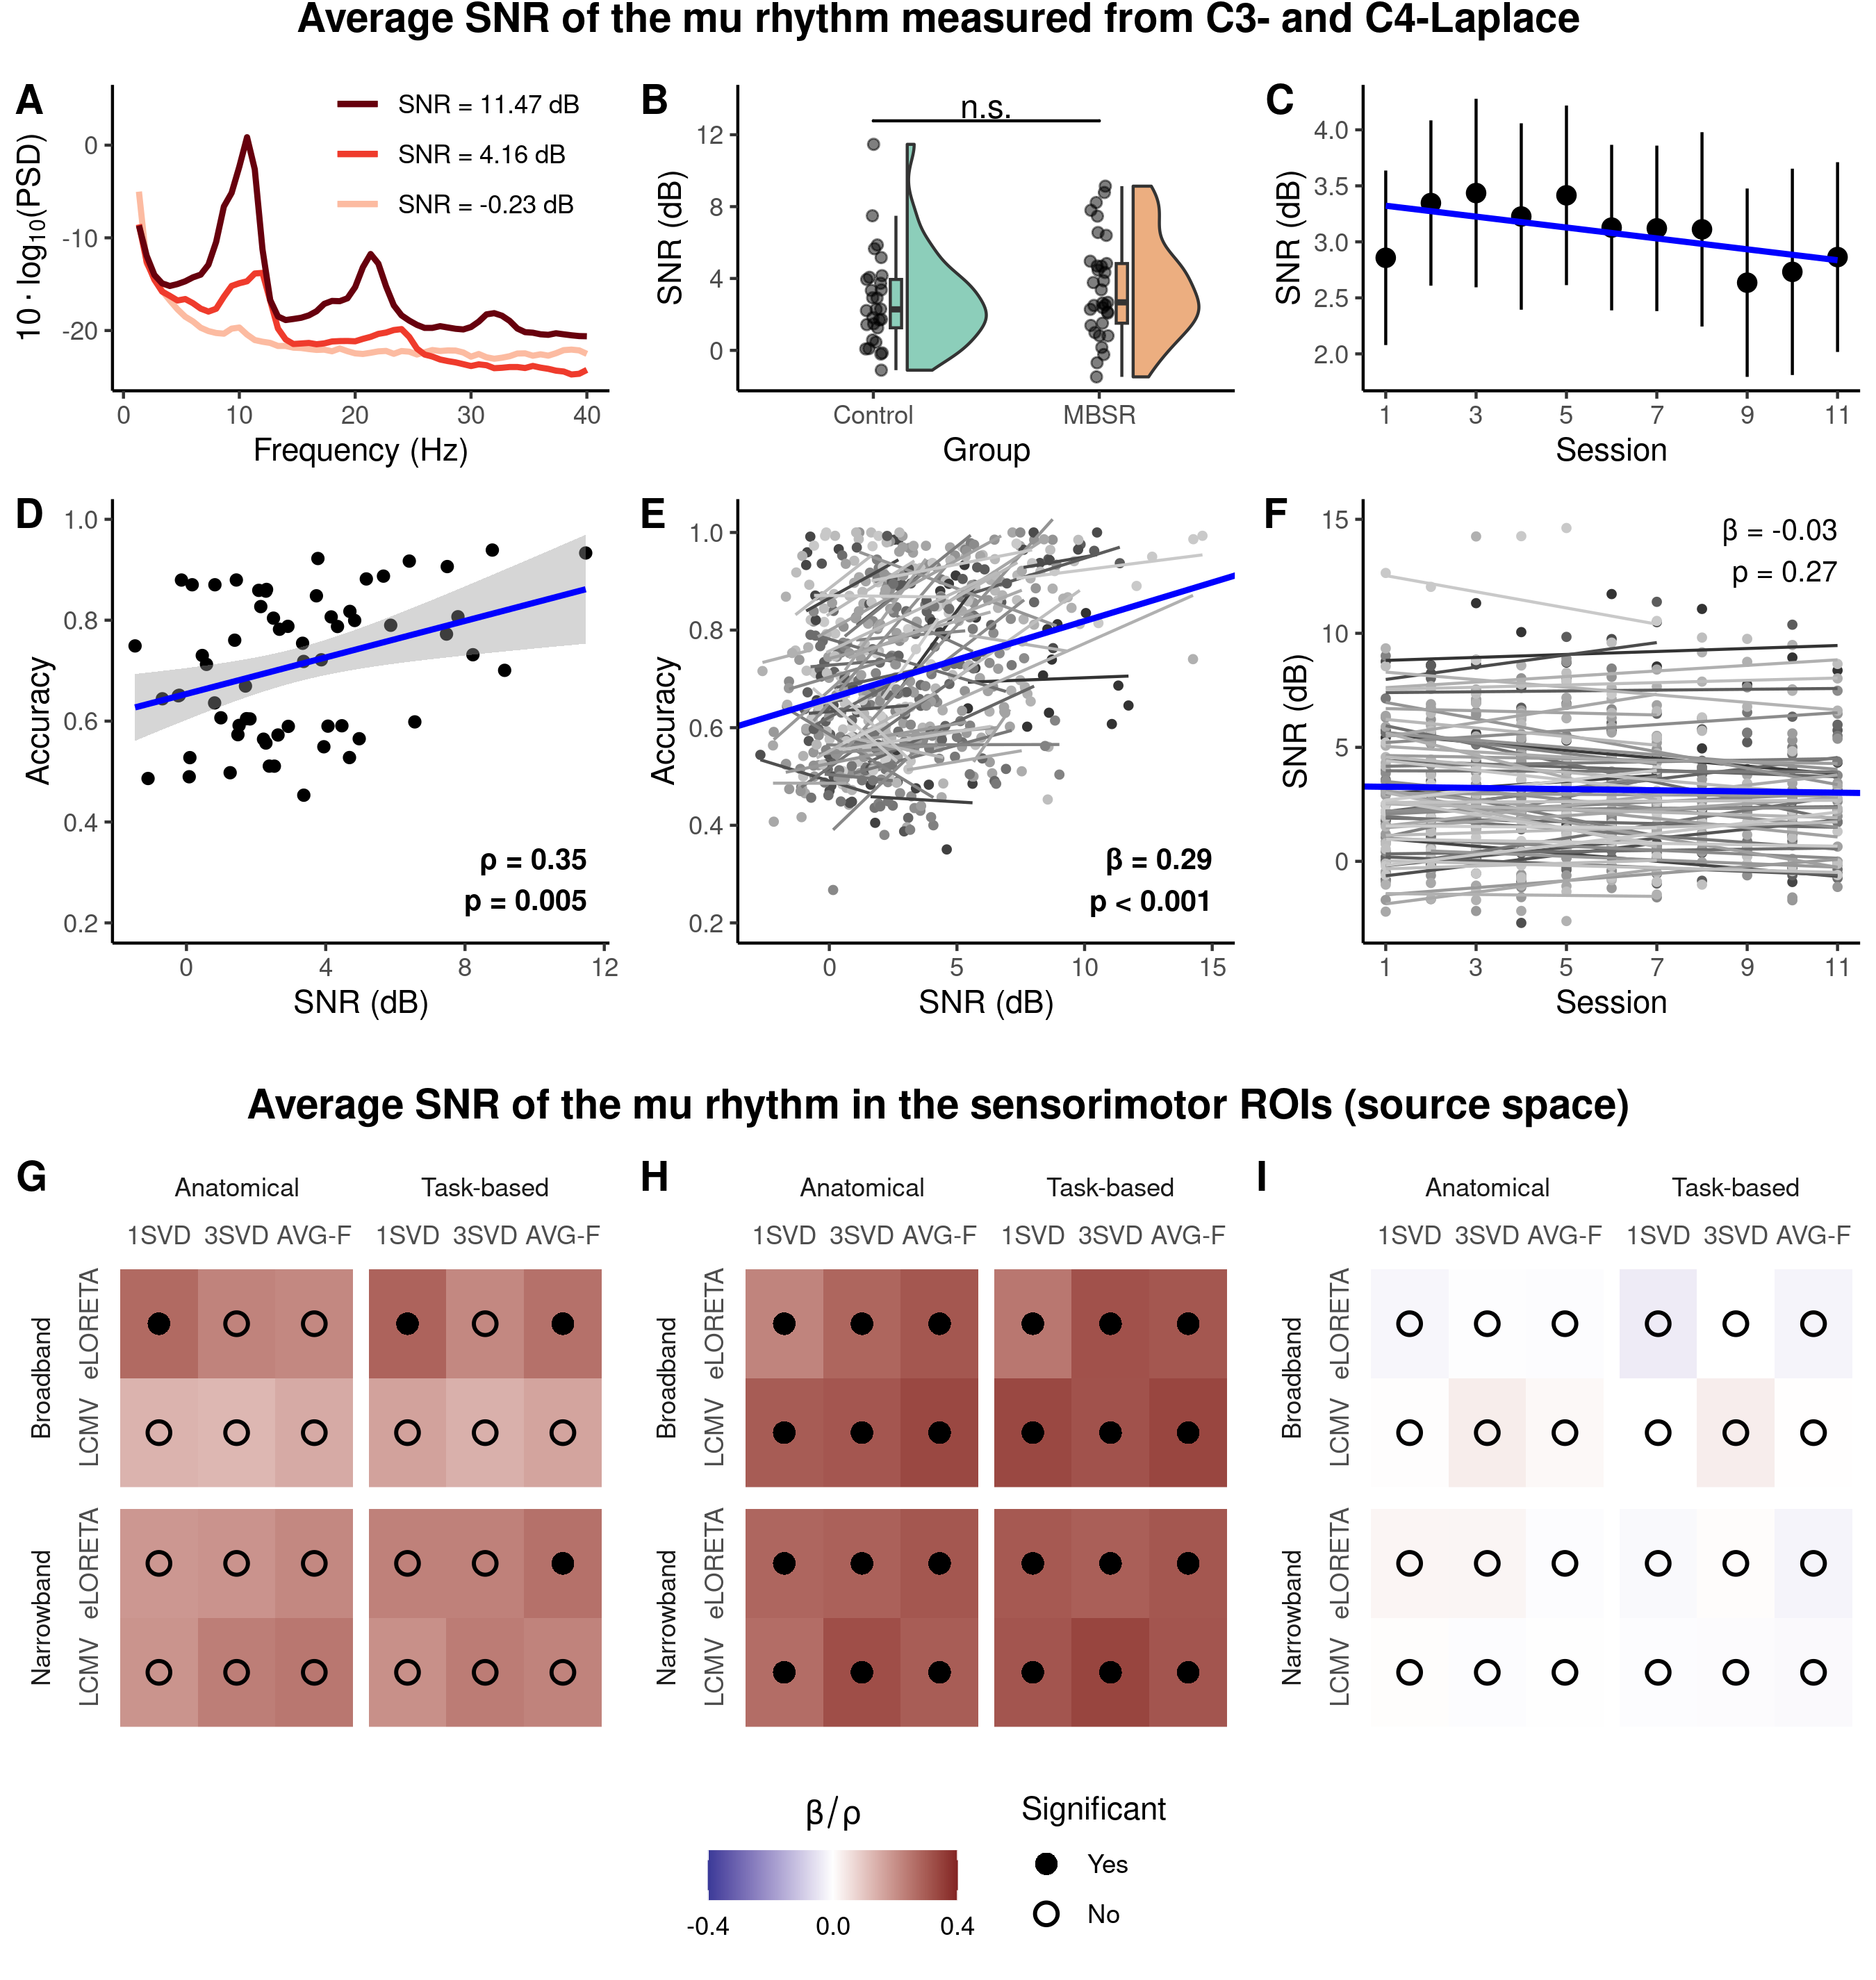
\includegraphics[width=\textwidth]{fig5-snr-rest-accuracy-session.png}
    \caption{Laplace and ROI SNR showed both between- and within-subject effects on BCI performance and did not change systematically throughout the training. (A) Examples of resting-state power spectra (average of C3- and C4-Laplace over all sessions) for representative subjects with different levels of Laplace SNR. (B) The difference in SNR between groups was not significant. (C) Dynamics of group-average SNR across sessions. (D) Accuracy positively correlated with SNR after averaging over all sessions. Each point corresponds to a single participant. (E) Within-subject variability of BCI performance was related to session-to-session changes in SNR. Each point corresponds to a single session. Within-subject (gray) and group-level (blue) linear trends are shown. (F) No longitudinal changes were observed for SNR. Within-subject (gray) and group-level (blue) linear trends are shown. Note the difference in y-axis scale compared to Panel C. (G) Multiverse analysis of between-subject correlation ($\rho$, coded with color) between ROI SNR and BCI performance. (H) Within-subject effect ($\beta$, coded with color) of ROI SNR on BCI performance in a multiverse analysis. (I) No evidence for longitudinal changes in ROI SNR was observed for all pipelines in the multiverse analysis. Fixed effect of session on ROI SNR ($\beta$) is coded with color.}
    \label{fig:snr_vs_accuracy_session_combined}
\end{figure}

\subsection{Effects of source space SNR, but not phase synchronization, were stable in the multiverse analysis}

In the source space analysis, we estimated values of ROI SNR and phase synchronization (PS) in sensorimotor brain areas and investigated their relationship to the BCI performance as well as changes throughout the training. We performed a multiverse analysis to investigate the robustness of the observed effects to the selection of the pipeline. Figures \ref{fig:snr_vs_accuracy_session_combined}G and \ref{fig:snr_vs_accuracy_session_combined}H show that the estimated effects of ROI SNR on accuracy were positive for all \numPipelines~pipelines both on the between- and within-subject levels, respectively. Additionally, on the within-subject level, all effects were significant. Figure \ref{fig:snr_vs_accuracy_session_combined}I shows that no significant longitudinal changes in ROI SNR were observed for all considered pipelines. Overall, the results of the multiverse analysis for ROI SNR corresponded to the results for Laplace SNR and showed that the selection of the pipelines did not affect the observed effect of ROI SNR on performance and changes in ROI SNR.

\medskip

For the PS, we first checked whether the grand-average spectra of within- and across-hemisphere values of PS measures show a pronounced peak in the mu frequency range. Such a peak indicates that the interaction is specific to the ongoing mu oscillations. As shown in Fig. \ref{fig:snr_connectivity}A for anatomical and Fig. \ref{supp-fig:multiverse_connectivity_spectra} for task-based definitions of ROIs, the peak was pronounced in most cases. However, within-hemisphere coherence estimated using the first SVD component showed almost identical values in the whole frequency range. In this case, it might occur due to the volume conduction, which equally affects all the frequencies.

\medskip

In line with the previous studies \citep{Bayraktaroglu2013, Vidaurre2020}, we observed a robust positive effect of ROI SNR on ImCoh and LagCoh, which are not sensitive to both spurious (caused by volume conduction) as well as genuine zero-lag interactions (Fig. \ref{fig:snr_connectivity}B). In contrast, the effects of ROI SNR on coherence were less consistent between pipelines and differed in sign depending on the selection of the processing methods. Overall, these results confirm that it is necessary to account for SNR in the analyses of effects related to PS.

\begin{figure}[htbp]
    \centering
    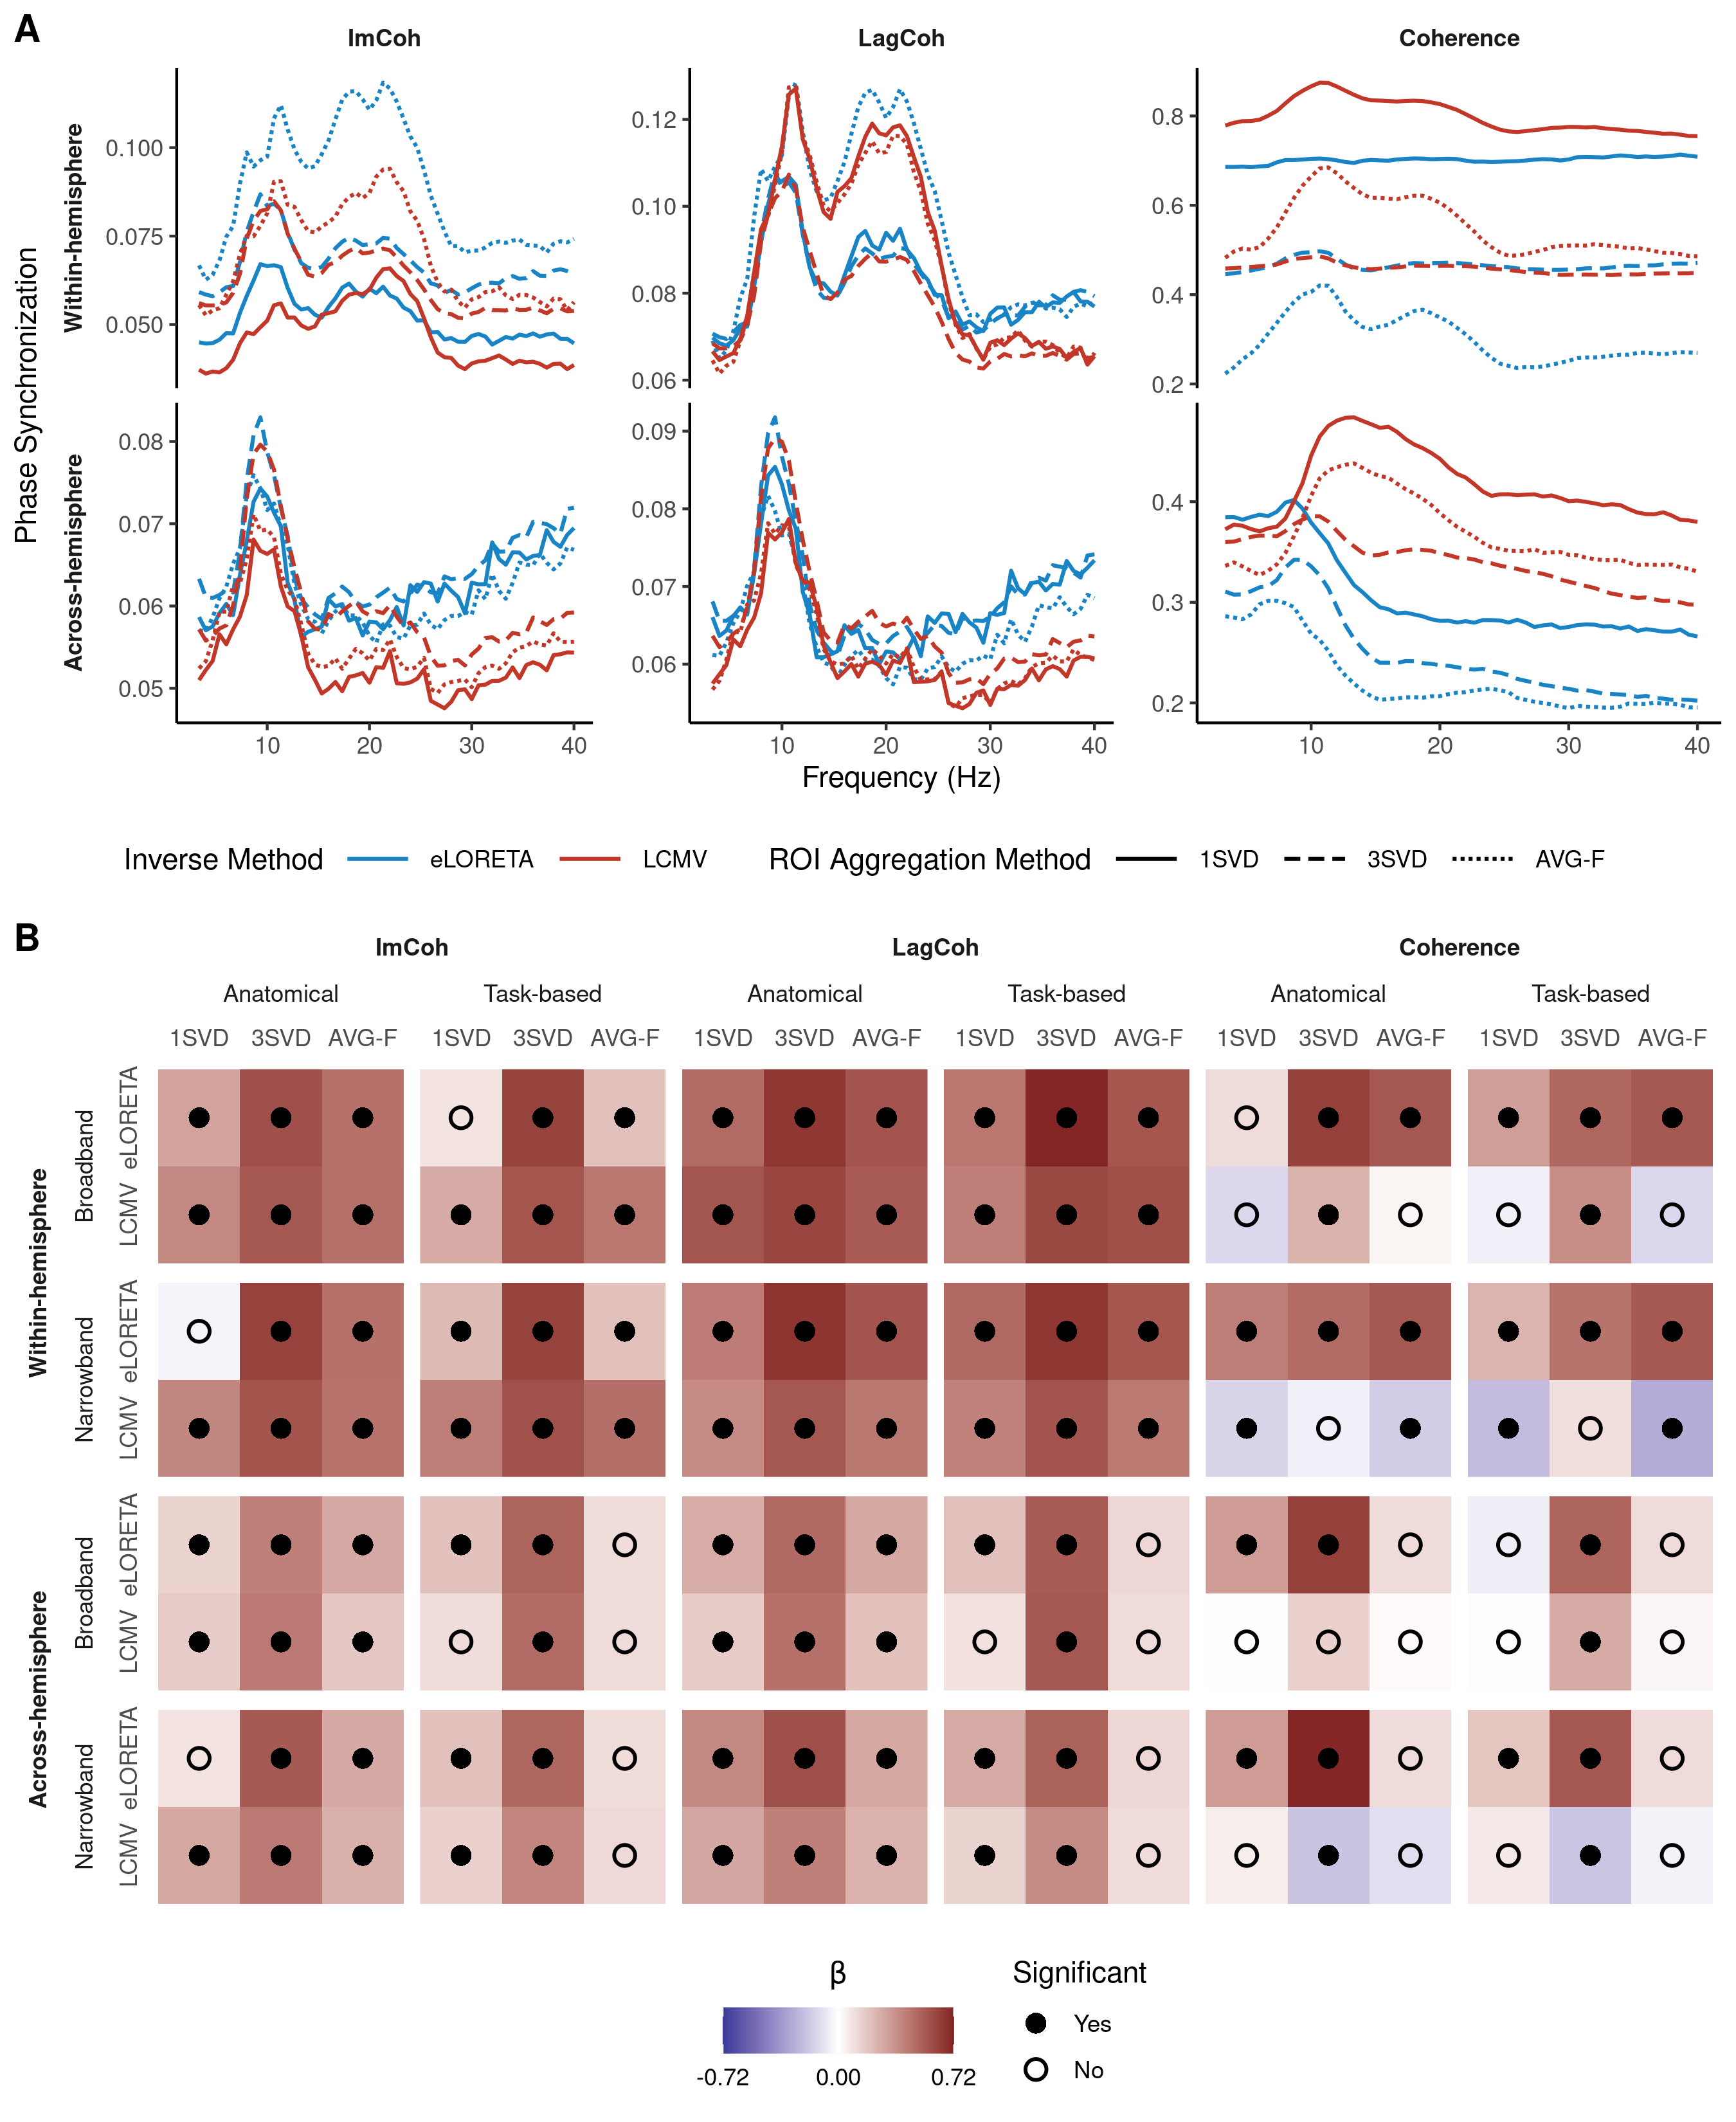
\includegraphics[width=\textwidth]{fig6-snr-connectivity.png}
    \caption{Multiverse analysis of the relationship between SNR and phase synchronization (PS) measures. (A) Grand average spectra of within- (top row) and across-hemisphere (bottom row) values of ImCoh, LagCoh, and coherence (columns: left to right) for the broadband pipelines with anatomical definitions of ROIs and different ROI aggregation methods. (B) ROI SNR showed consistent positive effects on ImCoh and LagCoh but not on coherence, both for within- and across-hemisphere PS. Fixed effect of ROI SNR on PS ($\beta$) is coded with color.}
    \label{fig:snr_connectivity}
\end{figure}

\medskip

Then, we investigated the relationship between PS and accuracy as well as changes in PS over time. For both research questions, effects were not significant for the majority of the pipelines and PS measures (Fig. \ref{fig:multiverse_connectivity_performance_within}). Nevertheless, the pipelines that led to significant results often corresponded to a choice of a particular method at different processing steps. For example, the effects of within-hemisphere ImCoh and LagCoh on accuracy were more likely to be significant when inverse modeling was performed with an LCMV beamformer (Fig. \ref{fig:multiverse_connectivity_performance_within}A, rows 2 and 4 from the top). In this case, pipeline-specific results showed up as stripes in the visualization. A different tendency was observed for the between-subject effect of PS on accuracy (Fig. \ref{supp-fig:multiverse_connectivity_performance_between}) as well as longitudinal changes in PS (Fig. \ref{supp-fig:multiverse_connectivity_longitude}): When assessing PS using coherence, significant effects were more likely to emerge than for other PS measures. Overall, the effects of connectivity on performance were not significant for the majority of the pipelines, and the direction of the effects was not consistent between different pipelines and PS measures.

\begin{figure}[htbp]
    \centering
    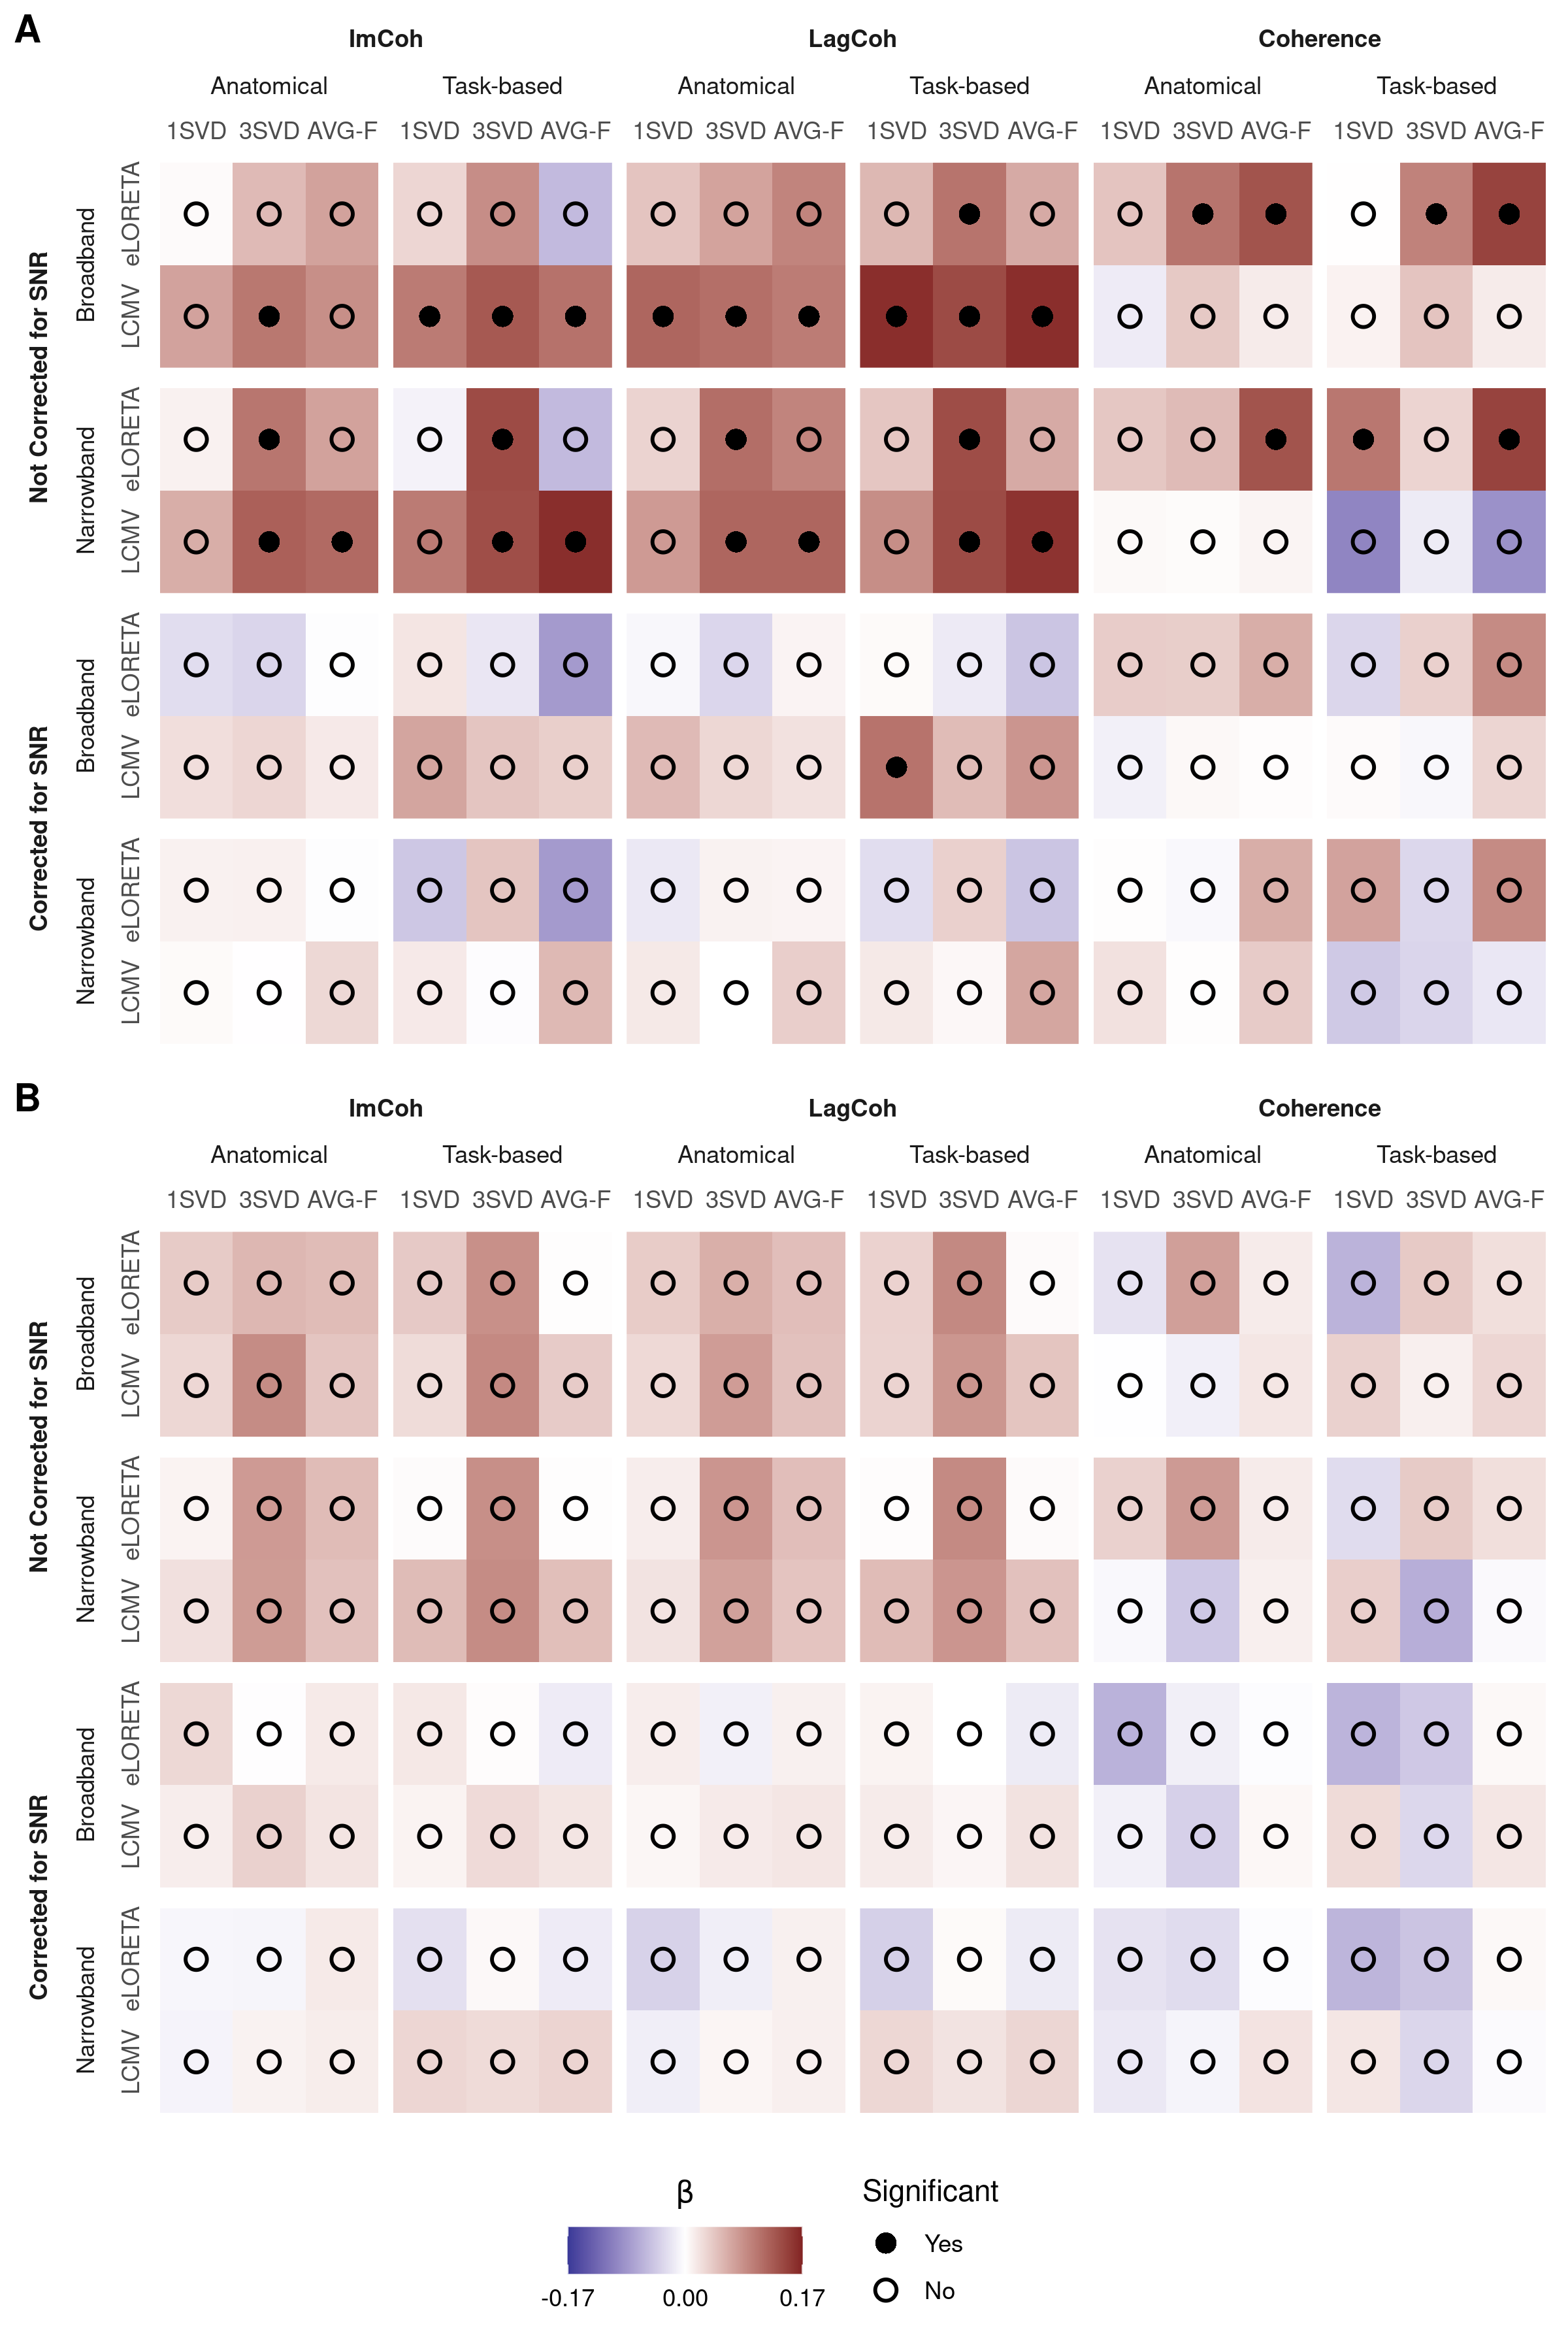
\includegraphics[width=0.925\textwidth]{fig7-multiverse-connectivity-performance-within.png}
    \caption{Within-subject effects of PS on BCI performance ($\beta$, coded with color) in the split multiverse analysis. Bonferroni correction for multiple ($m = \numComparisons$) comparisons was applied. Panels (A) and (B) correspond to within- and across-hemisphere PS, respectively.}
    \label{fig:multiverse_connectivity_performance_within}
\end{figure}

\medskip

Finally, we ran a joint analysis for all research questions by pooling together the data from all of the pipelines and fitting one linear mixed model per question (Fig. \ref{fig:multiverse_joint_analysis}). Once again, the aforementioned effects of ROI SNR on accuracy and PS were significant and robust to the selection of the pipeline. Effects of ImCoh and LagCoh on accuracy were significant before correction for ROI SNR but less consistent between considered pipelines. For ImCoh, the effect on accuracy remained significant in the joint analysis after correction for ROI SNR, but none of the pipelines showed the same effect in the split analysis (when a separate mixed model is fitted for each of the pipelines). Based on the evidence from all of the pipelines, across-hemisphere LagCoh and coherence significantly increased over the course of the training. However, for LagCoh longitudinal changes were significant only in two pipelines. Statistical results are presented in Table \ref{supp-tab:multiverse_effects_summary}. 

\begin{figure}[htbp]
    \centering
    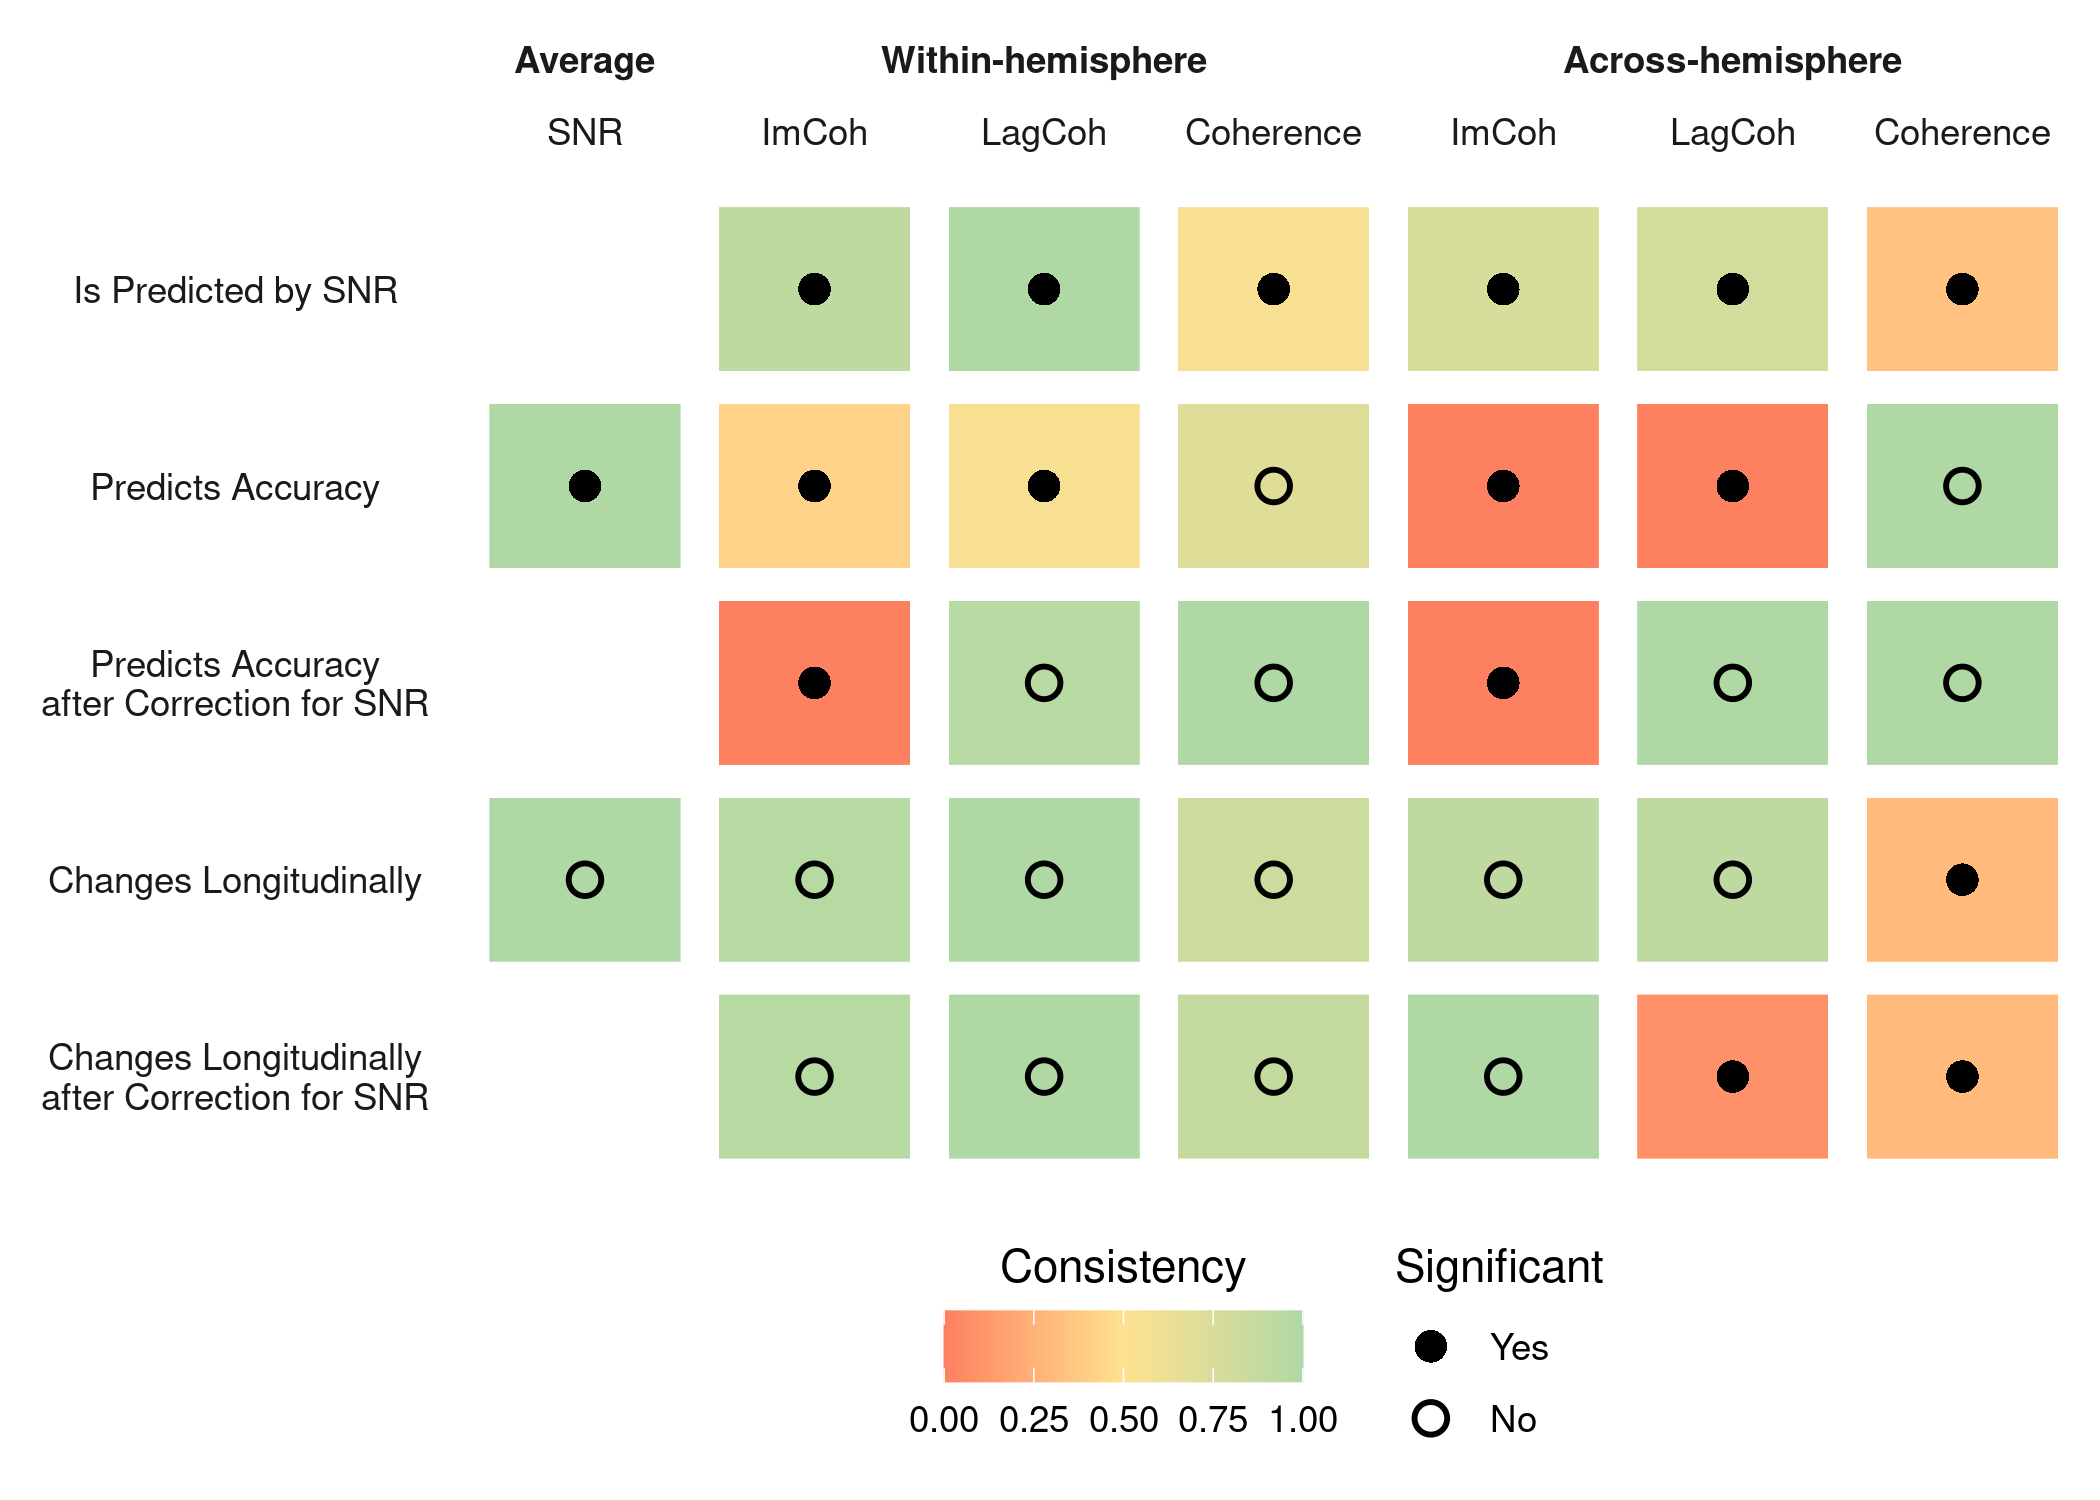
\includegraphics[width=0.9\textwidth]{fig8-multiverse-joint-analysis.png}
    \caption{Overview of the observed within-subject effects in the joint multiverse analysis. Bonferroni correction for multiple ($m=\numComparisons$) comparisons was applied to account for several PS measures. Color codes the number of pipelines that led to the same statistical result (and, if significant, the same direction of the effect) as the joint analysis.}
    \label{fig:multiverse_joint_analysis}
\end{figure}

\subsection{The selection of processing methods for the source space analysis affected the estimated values of SNR and PS}

Effects of different methods on the estimated values of ROI SNR and PS were assessed with a linear mixed model. We included fixed effects of all processing steps and all two-way interactions in the model to investigate whether the selection of the pipeline systematically affected the estimated values of SNR and PS. Table \ref{tab:pipeline_effects_summary} contains the estimated t-values for fixed effects of all predictors, while Table \ref{supp-tab:pipeline_effects_interactions} lists all two-way interactions that were significant. In both tables, significant effects are highlighted in bold, and stars indicate that the effects remained significant after the correction for multiple comparisons.

\medskip

First, we observed that the values of SNR were affected by filtering and the choice of the method for inverse modeling, with the interaction of these processing steps also being significant (Fig. \ref{fig:pipeline_effects_highlights}A). We investigated this result in more detail since the quality of the source reconstruction with LCMV depends on the SNR \citep{LCMV_VanVeen1997}, and SNR played an important role in the previous analyses. For this purpose, we compared values of SNR within pairs of pipelines, which differed only in the method for inverse modeling. As shown in Fig. \ref{supp-fig:snr_band_inverse}, LCMV led to higher SNR than eLORETA for broadband pipelines, and the difference was especially pronounced for low values of SNR. For narrowband pipelines, SNR was on average higher when eLORETA was used.

\medskip

PS measures were affected by the selection of methods for all processing steps except filtering. When 3SVD or AVG-F were used for the extraction of ROI time series as compared to 1SVD, coherence decreased (Fig. \ref{fig:pipeline_effects_highlights}, Panels C and F), while ImCoh increased compared to 1SVD (Fig. \ref{fig:pipeline_effects_highlights}, Panels B and E). Task-based definitions of ROIs led to a decrease in within-hemisphere ImCoh and LagCoh as well as across-hemisphere LagCoh and coherence. Additionally, for within-hemisphere PS, there was a significant interaction between the ROI definition and the method for extraction of ROI time series. In particular, pipelines with 3SVD were less affected by the definition of the ROI (Fig. \ref{supp-fig:coh_within_mask_roi_method}). Finally, LCMV led to smaller values of LagCoh and higher across-hemisphere coherence than eLORETA (Fig. \ref{fig:pipeline_effects_highlights}D).

\begin{table}[htbp]
    \small
    \centering
    \resizebox{\linewidth}{!}{\pipelineEffectsSummary}
    \caption{Summary of the observed fixed effects (t-values) of different processing methods on the estimated values of SNR and phase synchronization (PS). Significant effects are highlighted in bold, and stars indicate that the effects remained significant after Bonferroni correction for multiple ($m = \numComparisons$) comparisons. Columns correspond to different processing steps, and a positive t-value for $Y | X$ denotes that SNR or PS was higher when $Y$ was used compared to $X$. X $|$ SNR denotes that a correction for SNR was applied. WH and AH stand for within- and across-hemisphere, respectively.}
    \label{tab:pipeline_effects_summary}
\end{table}

\begin{figure}[htbp]
    \centering
    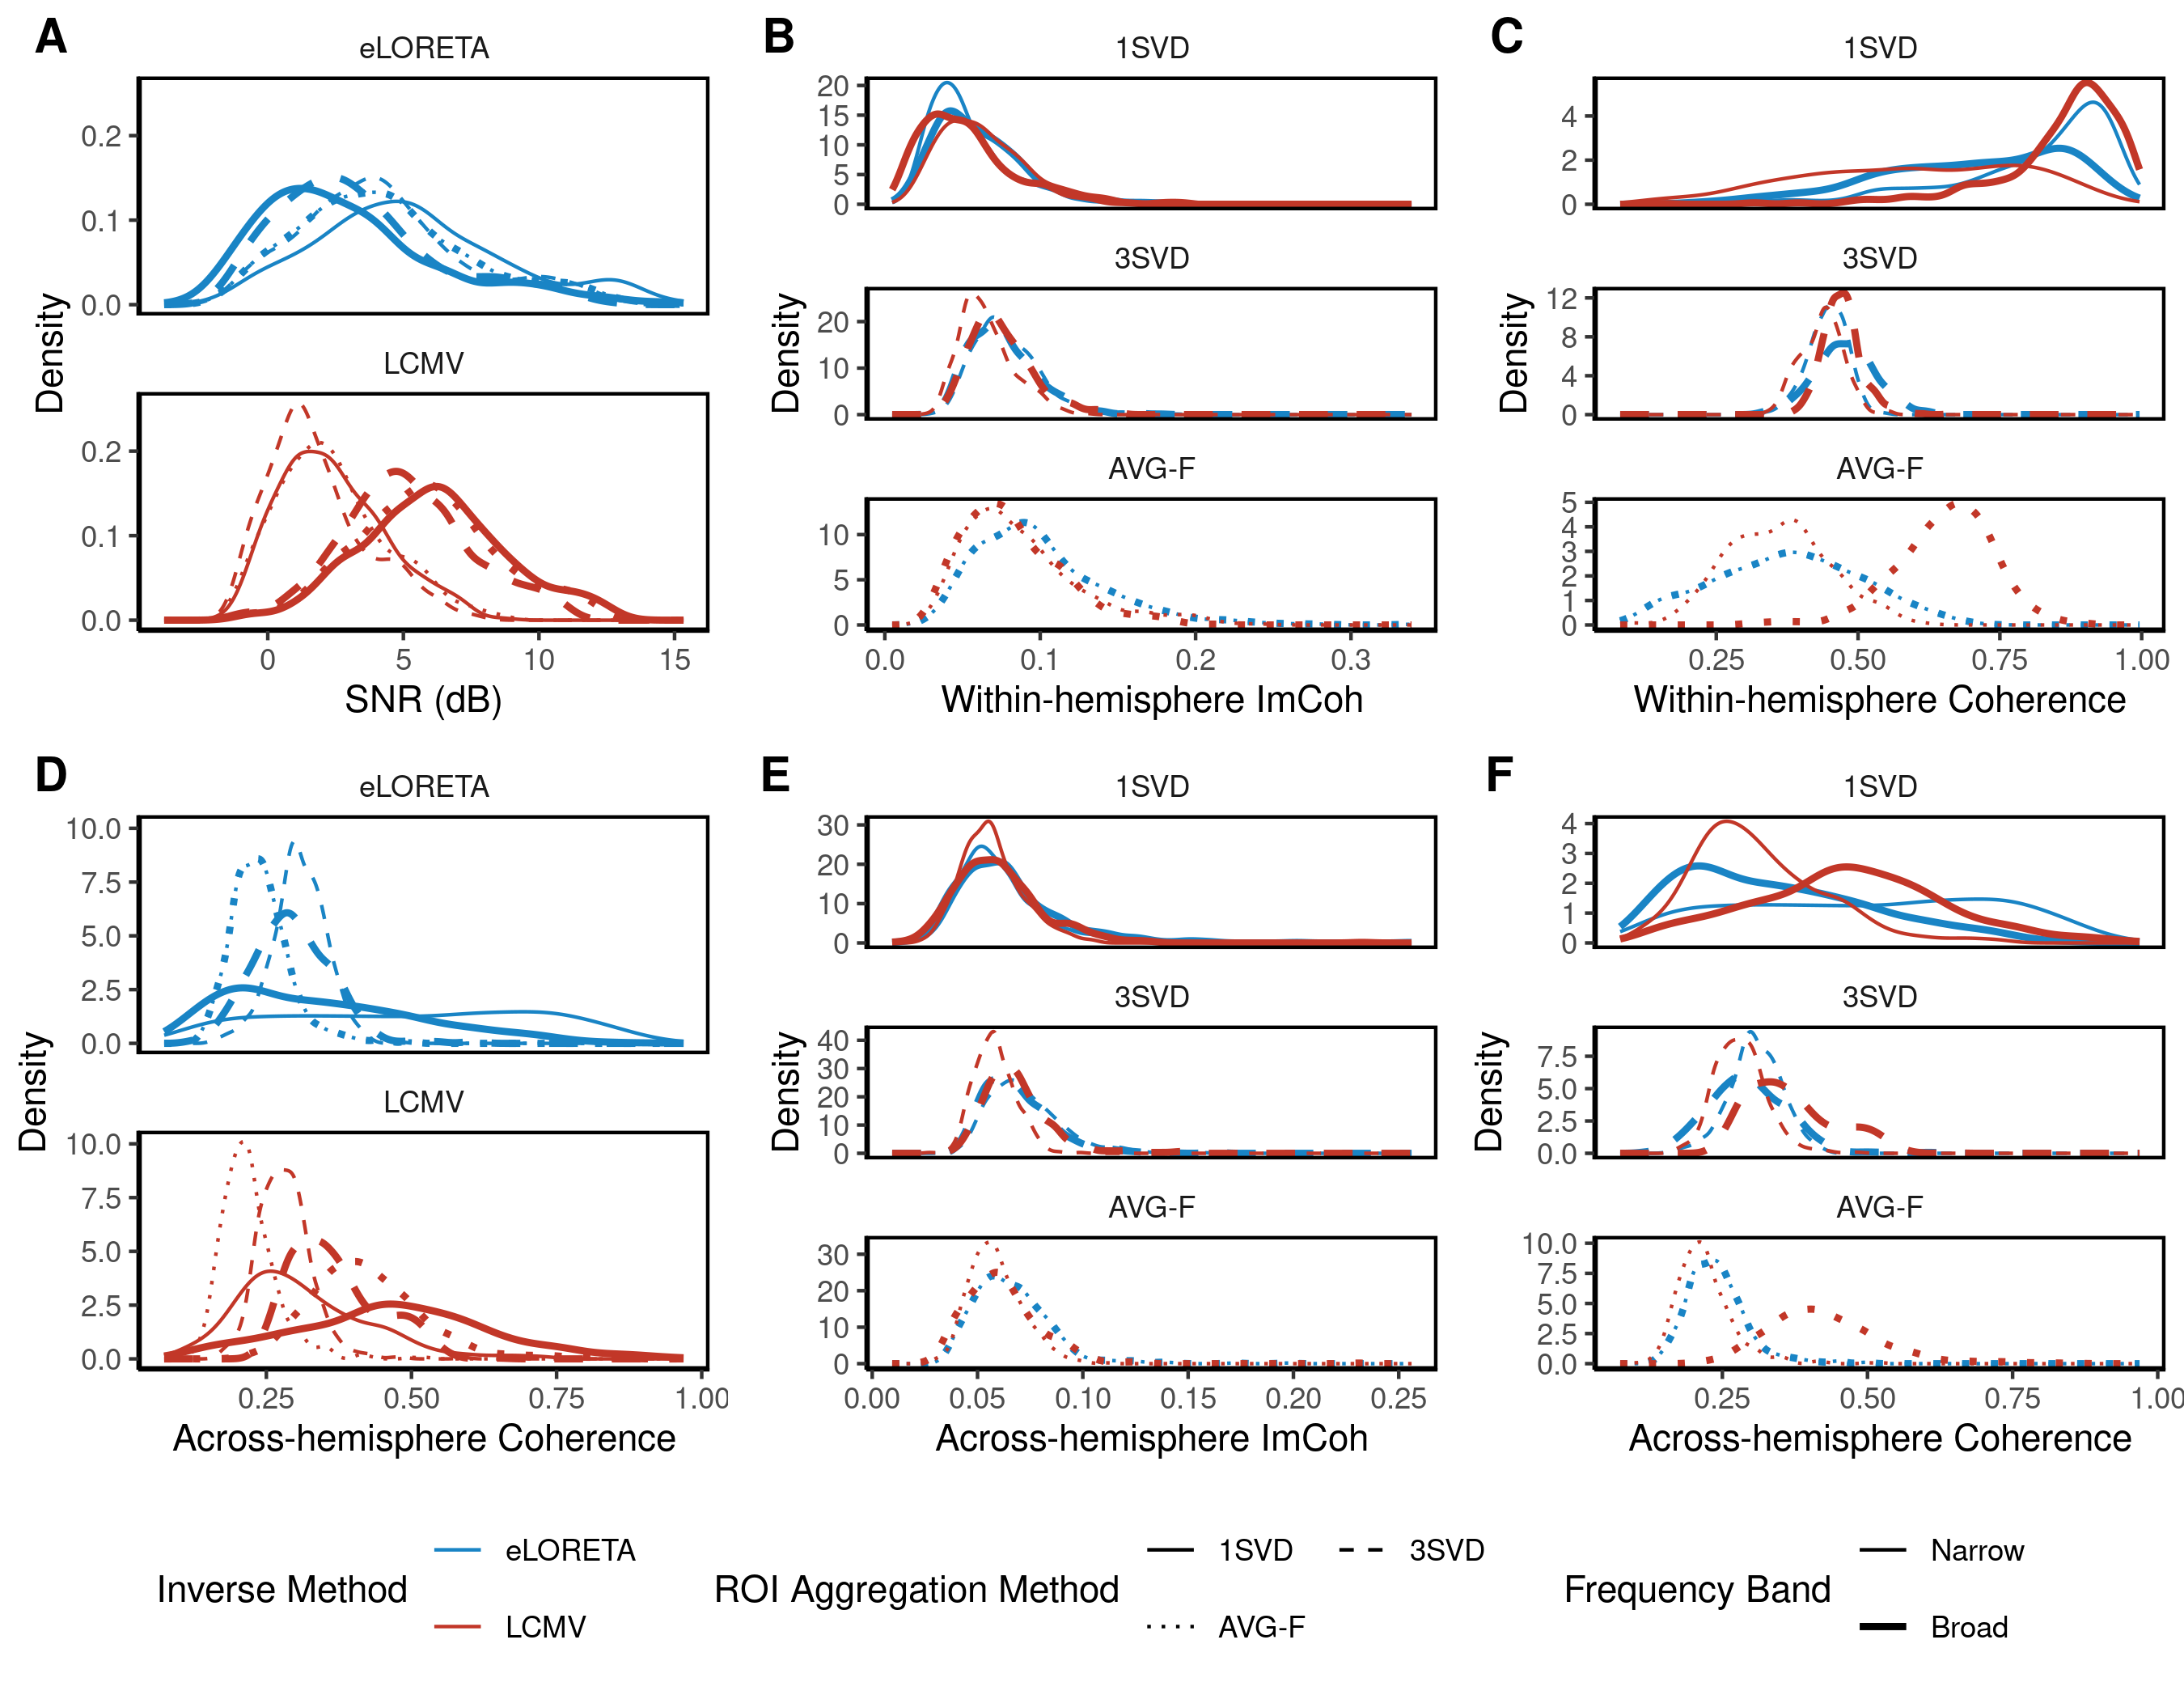
\includegraphics[width=\textwidth]{fig9-pipeline-effects-highlights.png}
    \caption{Selection of the processing methods affected estimated values of ROI SNR and PS as indicated by shifts in the empirical probability density functions. Only pipelines with anatomical definitions of ROIs are displayed. (A) SNR was affected by filtering and the choice of method for inverse modeling. (B) Within-hemisphere ImCoh was higher for 3SVD and AVG-F compared to 1SVD. (C) Method for extraction of ROI time series affected values of within-hemisphere coherence. (D) LCMV led to higher values of across-hemisphere coherence compared to eLORETA. (E) Same as B, but for across-hemisphere ImCoh. (F) Same as C, but for across-hemisphere coherence.}
    \label{fig:pipeline_effects_highlights}
\end{figure}
